% Section content template for individual Educative lessons
% This file contains the actual content for a specific section
% Generated from Educative API section content

% Section: Design Considerations of a Distributed Task Scheduler
% Section ID: 4856850956156928
% Section Slug: design-considerations-of-a-distributed-task-scheduler
% Generated: 2025-12-07T22:10:29.063425

\subsection{Queueing}\label{YZ6l8HexWqc_qOxufhB8C}
\\
A distributed queue is a major building block used by a scheduler. The simplest scheduling approach is to push the task into the queue on a \textbf{first-come, first-served basis}. If there are 10,000 nodes (resources) in a cluster (cloud), the task scheduler quickly extracts tasks from the queue and schedules them on the nodes. But, if all the resources are currently busy, then tasks will need to wait in the queue, and small tasks might need to wait longer.
\\
This scheduling mechanism can affect the reliability of the system, availability of the system, and priority of tasks. There could be cases where we want urgent execution of a task---for example, a task that notifies a user that their account was accessed from an unrecognized device. So , we can't rely only on the first-come, first-serve to schedule tasks. Instead
, we categorize the tasks and set appropriate priorities. We have the following three categories for our tasks:

\begin{itemize}
\item
\protect\phantomsection\label{01dKSikTm6xeg9huVKABK}
Tasks that can't be delayed.
\item
\protect\phantomsection\label{JyZx7ONlr_ZS3wTo_yjSS}
Tasks that can be delayed.
\item
\protect\phantomsection\label{Uvuzk7q5FENwuh07E_okP}
Tasks that need to be executed periodically (for example, every 5 minutes, or every hour, or every day).
\end{itemize}

\begin{figure}[htbp]
 \centering
 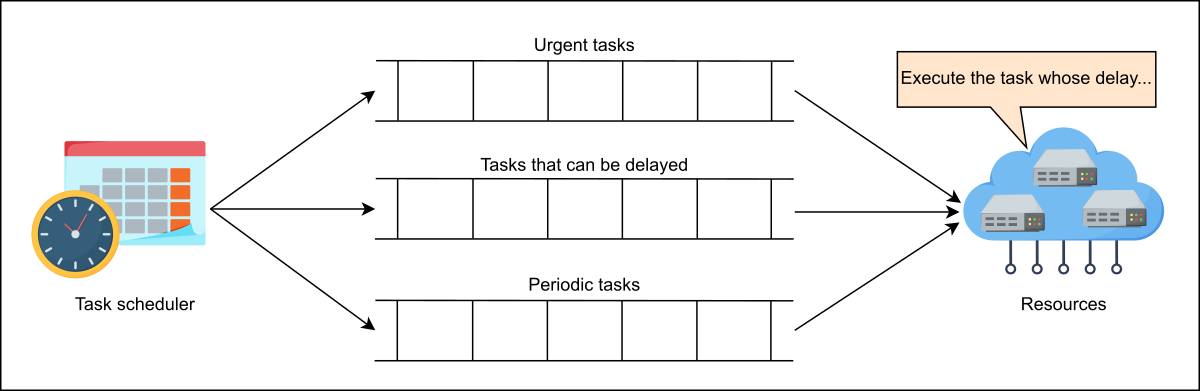
\includegraphics[width=0.5\textwidth]{Images/chapter_23/section_4856850956156928/5978174511251456.png}
 \caption{Multiple queues based on the task categories}
\end{figure}

Our system ensures that tasks in non-urgent queues are not starved. As soon as some task's delay limit is about to be reached, it is moved to the urgent tasks queue so that it gets service. We 'll see how the task scheduler implements priorities later in this lesson.
\\
Let's explore some parameters that help the scheduler efficiently utilize resources and provide reliable service to the users.

\subsection{Execution cap}\label{hna1b4aM2Yd9h_o-RgoC1}
\\
Some tasks take very long to execute and occupy the resource blocking other tasks. The \textbf{execution cap} is an important parameter to consider while scheduling tasks. If we completely allocate a resource to a single task and wait for that task's completion, some tasks might not halt because of a bug in the task script that doesn't let it finish its execution. We let the clients set the execution cap for their tasks. After that specified time, we should stop task execution, release the resource, and allocate it to the next task in the queue. If the task execution stops due to the execution cap limit, our system notifies the respective clients of these instances. The client needs to do appropriate remedial actions for such cases.
\\
If clients don't set the execution cap, the scheduler uses its default upper bound on the maximum allowed time to kill the tasks. Suppose a task actually takes longer---for example, if we are training a machine learning model. In that case, the scheduler might need to pause and resume a task many times to accommodate other tasks. It wouldn't be fair to the short task that has to wait for two days to use a resource for two seconds.
\\
Cloud providers can't let a task execute for an unlimited time for a basic (free) account, because using their resources costs a certain fee to the providers. To handle such cases, clients are informed about maximum usage limits so that they can handle long task execution. For example, clients may design their task in such a way that they checkpoint after some time and load from that state to resume progress in case resources are taken from the client due to usage limit.

\begin{quote}
\textbf{Quiz:}
\textbf{Question 1:} What if a long task is 90\% executed, but before it completes, the machine that was executing this task fails?
\textbf{Answer:} The task scheduler will re-execute the task on some other machine. Tasks need to be either idempotent, which is discussed later in the lesson, or they should be able to restore their state from a previous checkpoint.

Once the state is saved, we can resume that task's execution on any other machine. This makes our system fault tolerant and saves our resources.
\end{quote}

\subsection{Prioritization}\label{-pd9k1vUO3ClZyGXWenpF}
\\
There are tasks that need urgent execution. For example, in a social application like Facebook, the users can mark themselves safe during an emergency situation, such as an earthquake. The tasks that carry out this activity should be executed in a timely manner, otherwise this feature would be useless to Facebook users. Sending an email notification to the customers that their account was debited a certain amount of money is another example of tasks that require urgent execution.
\\
To prioritize the tasks, the task scheduler maintains a \textbf{delay tolerance} parameter for each task and executes the task close to its delay tolerance. \textbf{Delay tolerance} is the maximum amount of time a task execution could be delayed. The task that has the shortest delay tolerance time is executed first. By using a delay tolerance parameter, we can postpone the tasks with longer delay tolerance values to make room for urgent tasks during peak times.

\begin{quote}
\textbf{Quiz:}
\textbf{Question 1:} How do we determine the value of delay tolerance?
\textbf{Answer:} Since there are different categories of tasks in various applications,

the application owners or clients can set or automate the values themselves, depending upon the task category. For example, in a social media application like Facebook, we can generate a newsfeed, suggest friends, allow users to mark themselves safe after a disaster, send notifications about a live stream event, and many more. Out of the listed tasks, the priority tasks should be to mark a person safe during an earthquake and send notifications about live stream events. Clients can tighten the delay tolerance values of these tasks down to milliseconds or a few seconds while tasks like suggesting friends can be delayed for days. The task scheduling system itself can set the delay tolerance value depending on the task category and its severity. There are different costs for different priorities (there are usually higher costs for high-priority tasks, for example) so that customers can carefully categorize their tasks.
\end{quote}

\subsection{Resource capacity optimization}\label{m88VcC5TeEA0Um9RReogl}
\\
There could be a time when resources are close to the overload threshold (for example, above 80\% utilization). This is called \textbf{peak time}. The same resource may be idle during off-peak times. So, we have to think about better utilization of the resources during off-peak times and how to keep resources available during peak times.
\\
There are tasks that don't need urgent execution. For example, in a social application like Facebook, suggesting friends is not an urgent task. We can make a separate queue for tasks like this and execute them in off-peak times. If we consistently have more work to do than the available resources, we might have a capacity problem, and to solve that, we should commission more resources. A cloud provider needs to have a target \textbf{resources-to-demand} ratio. When demand starts increasing, the ratio will move towards 0. If the ratio starts changing over time, the provider might decide to commission more or fewer resources.

\subsection{Task idempotency}\label{78_7qZ_iNU_fhJnwaA5MY}
\\
If the task executes successfully, but for some reason the machine fails to send an acknowledgement, the scheduler will schedule the task again. The task is executed again, and we end up with the wrong result, which means the task was non-idempotent. An example of non-idempotence is shown in the following illustration:

\begin{figure}[htbp]
 \centering
 \begin{subfigure}[b]{0.48\textwidth}
 \centering
 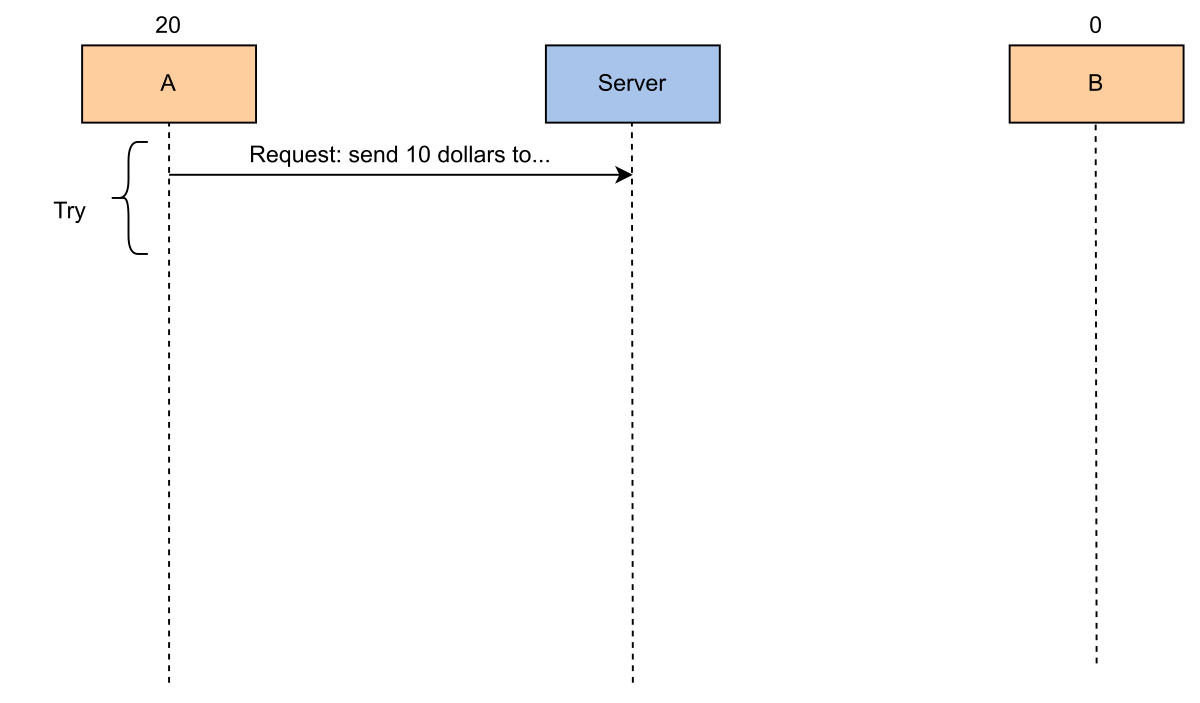
\includegraphics[width=\textwidth]{Images/chapter_23/section_4856850956156928/4783657135112192.png}
 \caption{A has 20 dollars. It makes a request to send 10 dollars to B, which has 0 dollars. A is the sender, and B is the receiver}
 \end{subfigure}
 \hfill
 \begin{subfigure}[b]{0.48\textwidth}
 \centering
 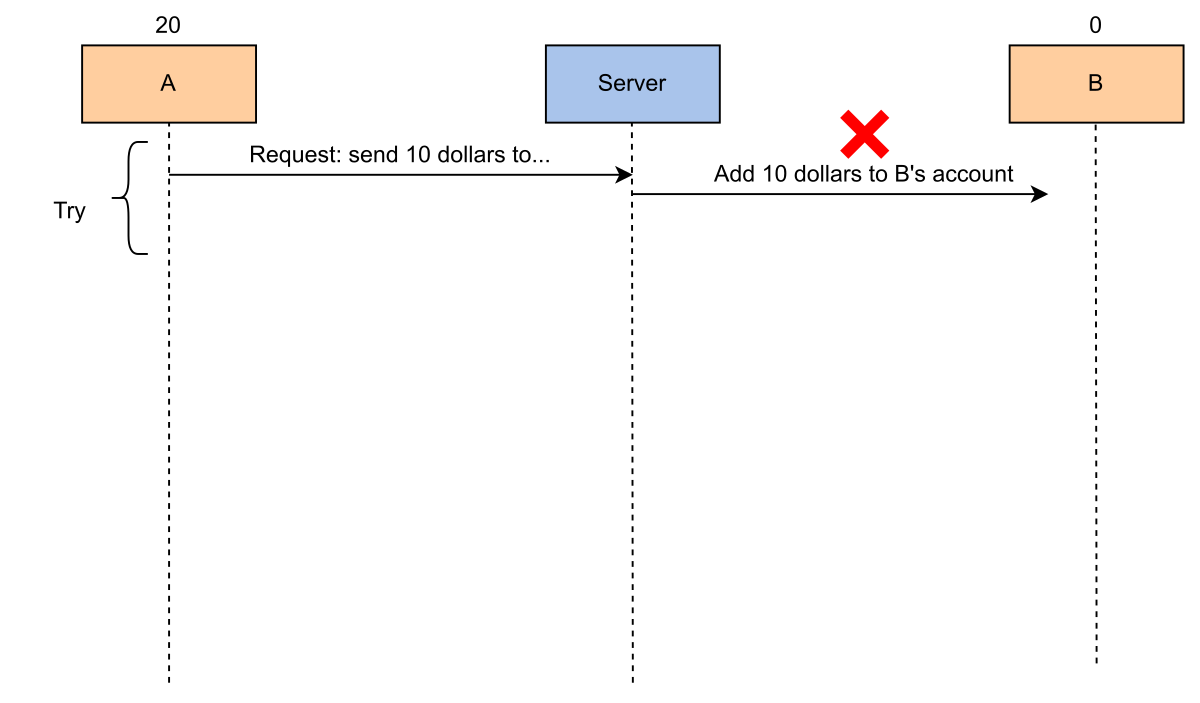
\includegraphics[width=\textwidth]{Images/chapter_23/section_4856850956156928/5068195350446080.png}
 \caption{ The server starts the operation of adding 10 dollars to B’s account, which doesn’t execute successfully}
 \end{subfigure}
\end{figure}

\begin{figure}[htbp]
 \centering
 \begin{subfigure}[b]{0.48\textwidth}
 \centering
 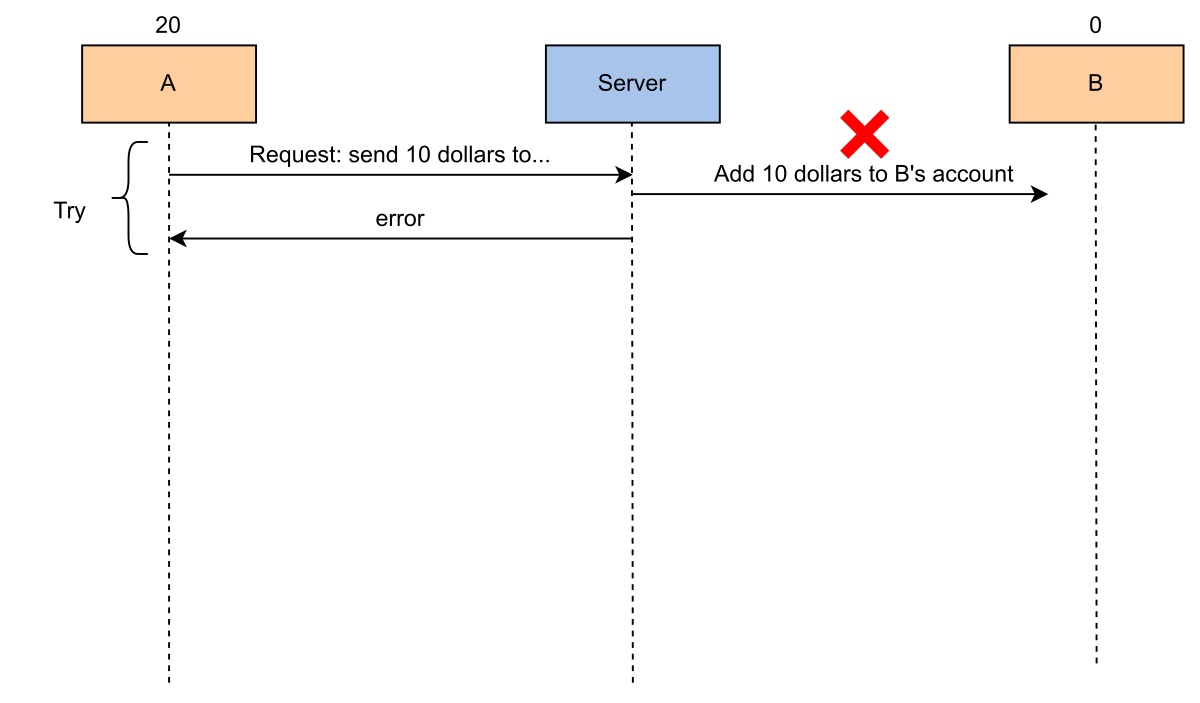
\includegraphics[width=\textwidth]{Images/chapter_23/section_4856850956156928/6063498467737600.png}
 \caption{The server sends an error message to A}
 \end{subfigure}
 \hfill
 \begin{subfigure}[b]{0.48\textwidth}
 \centering
 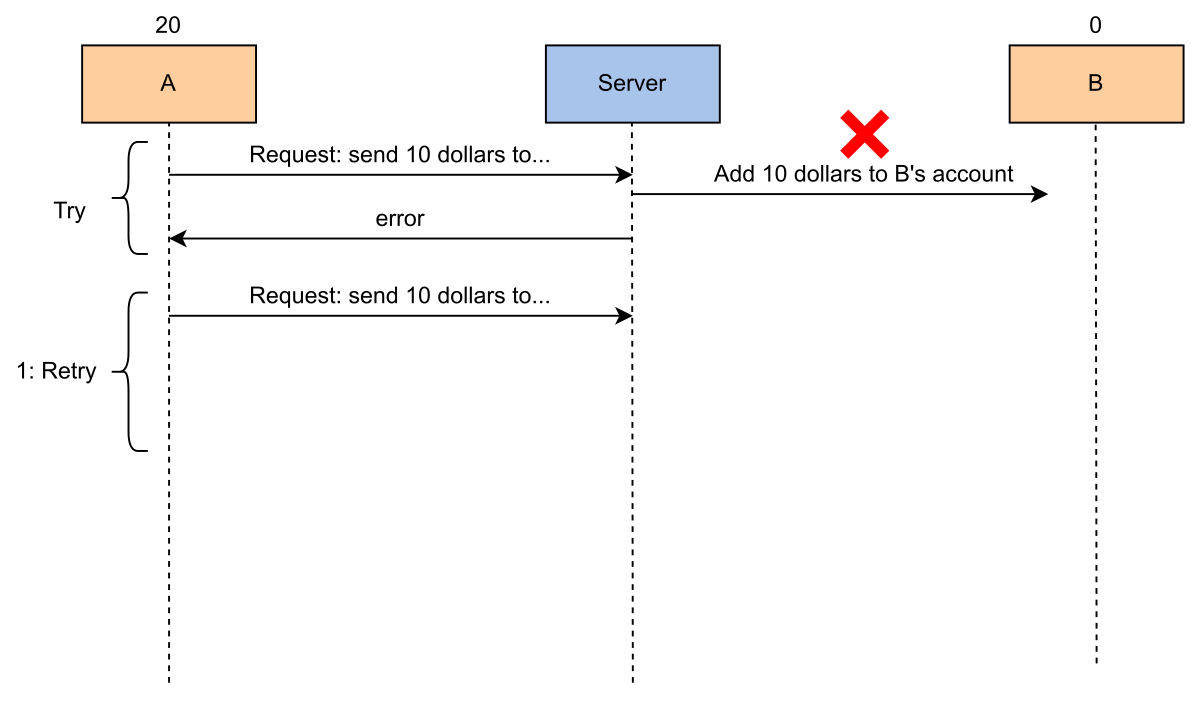
\includegraphics[width=\textwidth]{Images/chapter_23/section_4856850956156928/5971969023672320.png}
 \caption{A retries the transaction}
 \end{subfigure}
\end{figure}

\begin{figure}[htbp]
 \centering
 \begin{subfigure}[b]{0.48\textwidth}
 \centering
 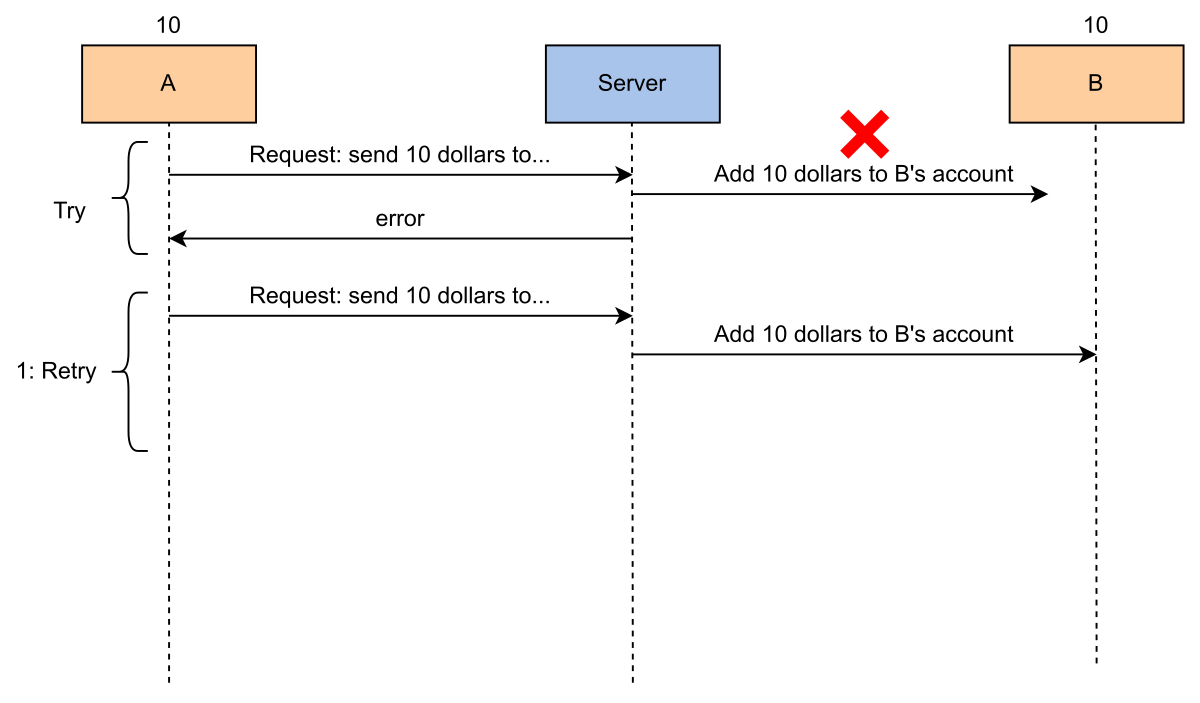
\includegraphics[width=\textwidth]{Images/chapter_23/section_4856850956156928/6555042564014080.png}
 \caption{The server starts the operation of adding 10 dollars to B’s account}
 \end{subfigure}
 \hfill
 \begin{subfigure}[b]{0.48\textwidth}
 \centering
 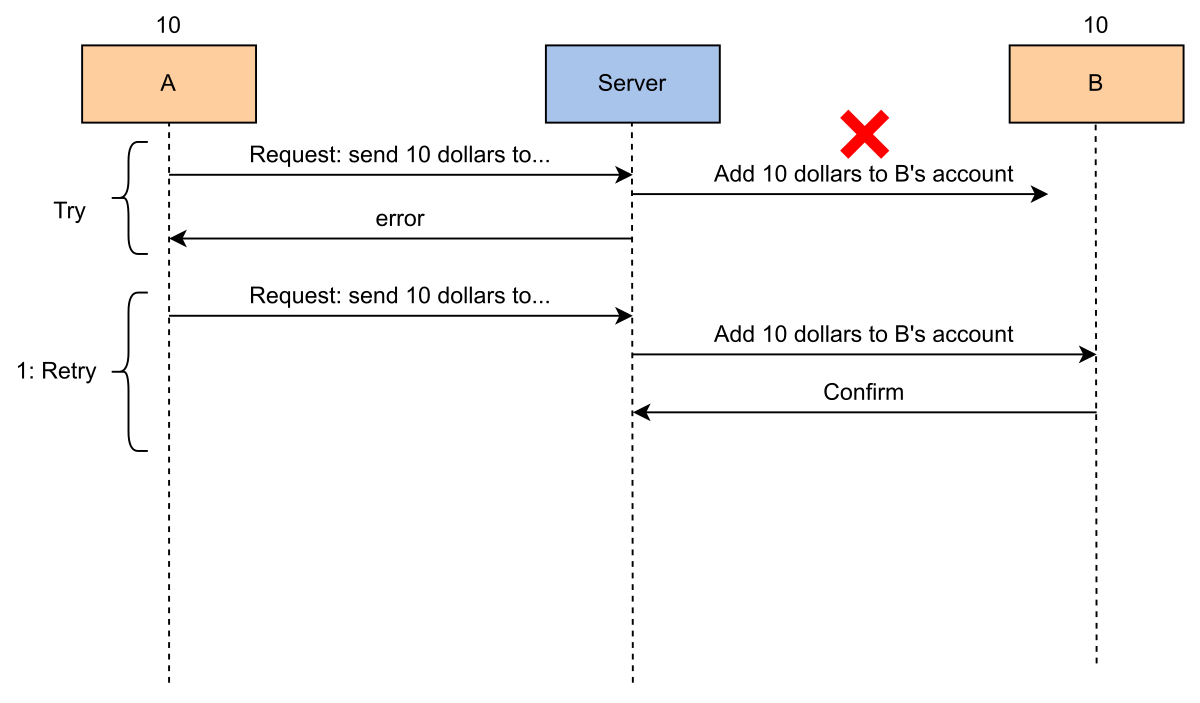
\includegraphics[width=\textwidth]{Images/chapter_23/section_4856850956156928/5373922006794240.png}
 \caption{This time server is able to execute the operation of adding 10 dollars to B’s account successfully, and B's balance is updated}
 \end{subfigure}
\end{figure}

\begin{figure}[htbp]
 \centering
 \begin{subfigure}[b]{0.48\textwidth}
 \centering
 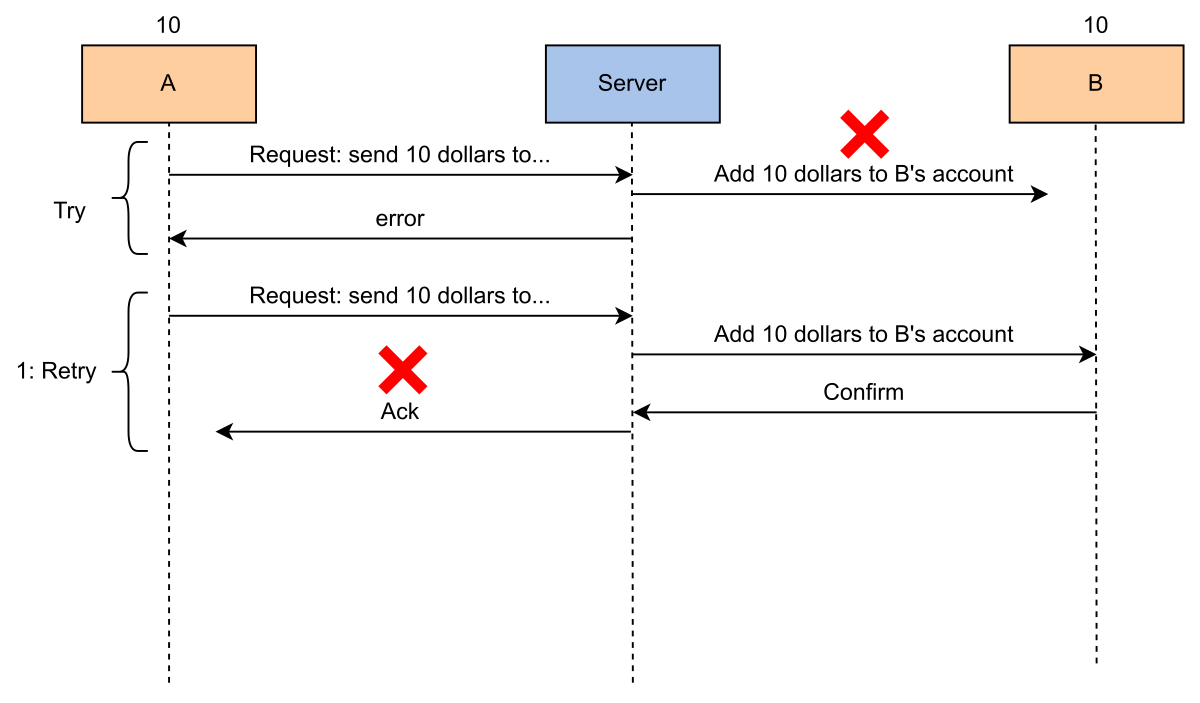
\includegraphics[width=\textwidth]{Images/chapter_23/section_4856850956156928/6213290674094080.png}
 \caption{The server sends an acknowledgment to A, but it couldn’t happen due to some error}
 \end{subfigure}
 \hfill
 \begin{subfigure}[b]{0.48\textwidth}
 \centering
 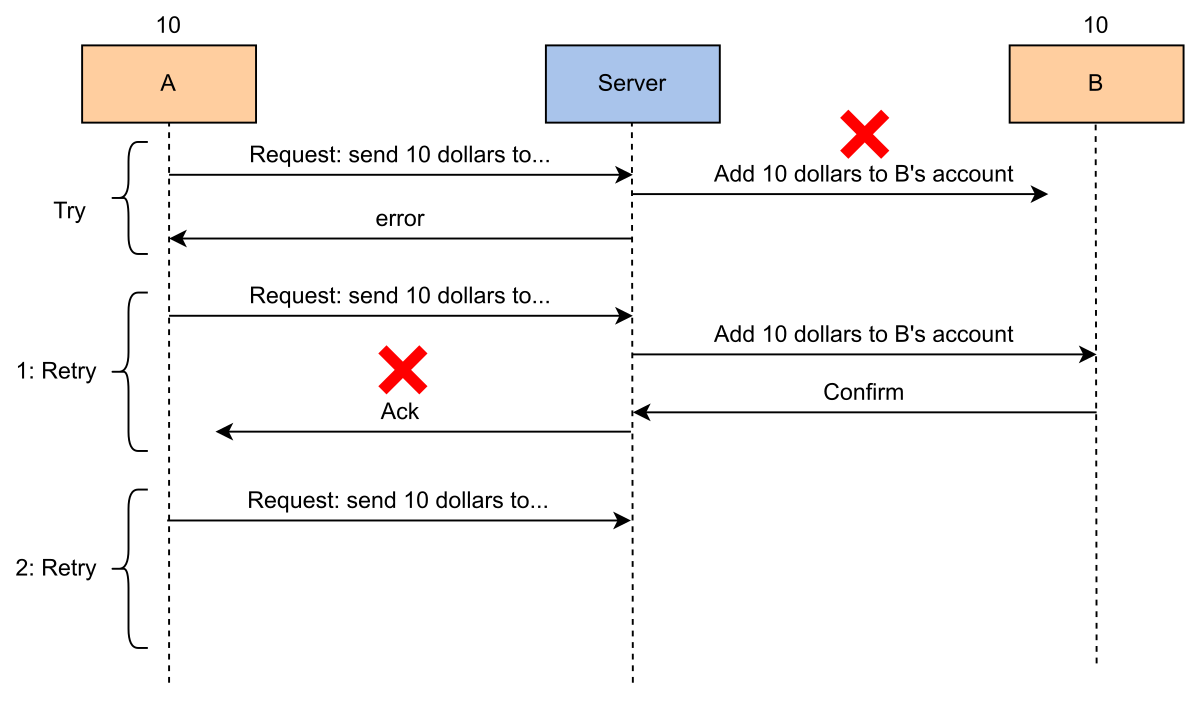
\includegraphics[width=\textwidth]{Images/chapter_23/section_4856850956156928/5859669050654720.png}
 \caption{A re-retries the transaction}
 \end{subfigure}
\end{figure}

\begin{figure}[htbp]
 \centering
 \begin{subfigure}[b]{0.48\textwidth}
 \centering
 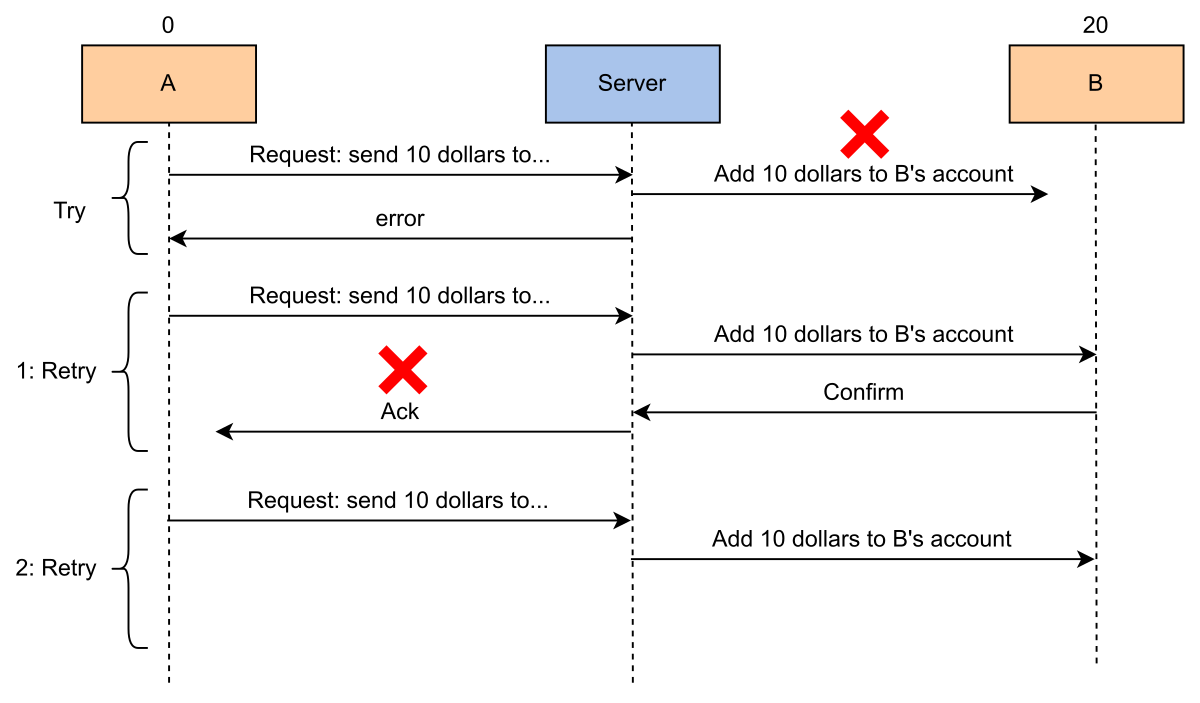
\includegraphics[width=\textwidth]{Images/chapter_23/section_4856850956156928/4663933042688000.png}
 \caption{Servers start the operation of adding 10 dollars to B’s account again}
 \end{subfigure}
 \hfill
 \begin{subfigure}[b]{0.48\textwidth}
 \centering
 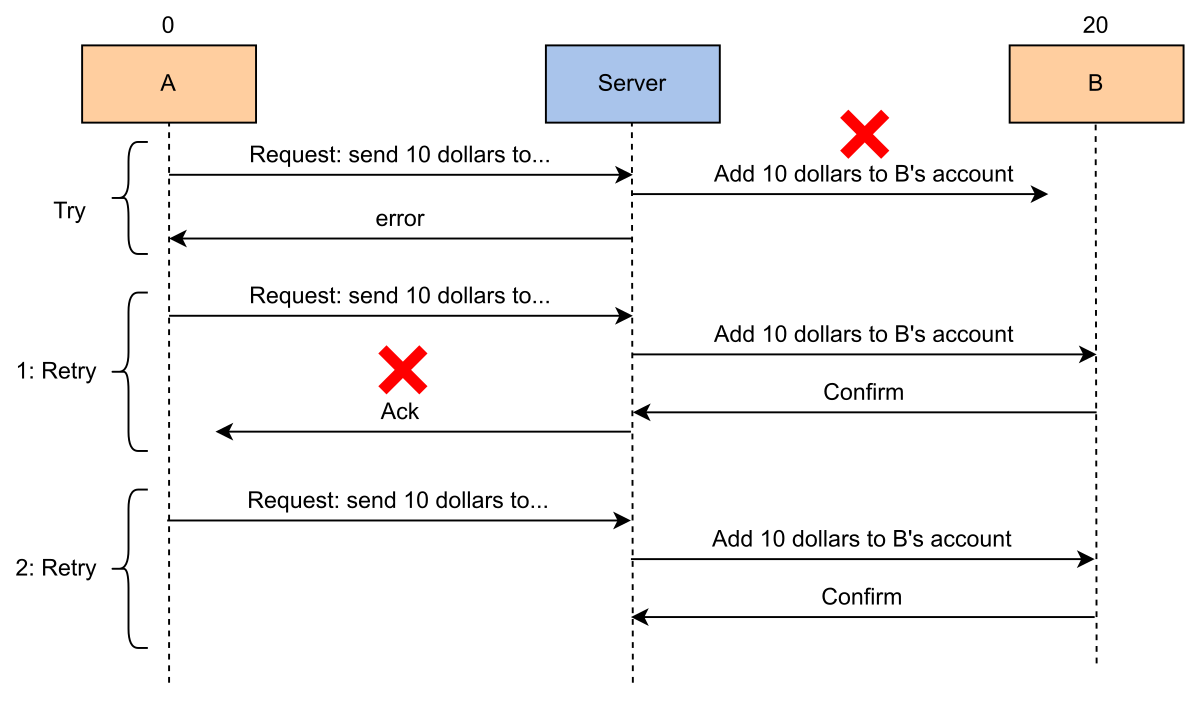
\includegraphics[width=\textwidth]{Images/chapter_23/section_4856850956156928/4951005334863872.png}
 \caption{The operation of adding 10 dollars to B’s account is executed successfully, and 10 dollars are added to B’s account again. B’s balance has changed to 20}
 \end{subfigure}
\end{figure}

\begin{figure}[htbp]
 \centering
 \begin{subfigure}[b]{0.48\textwidth}
 \centering
 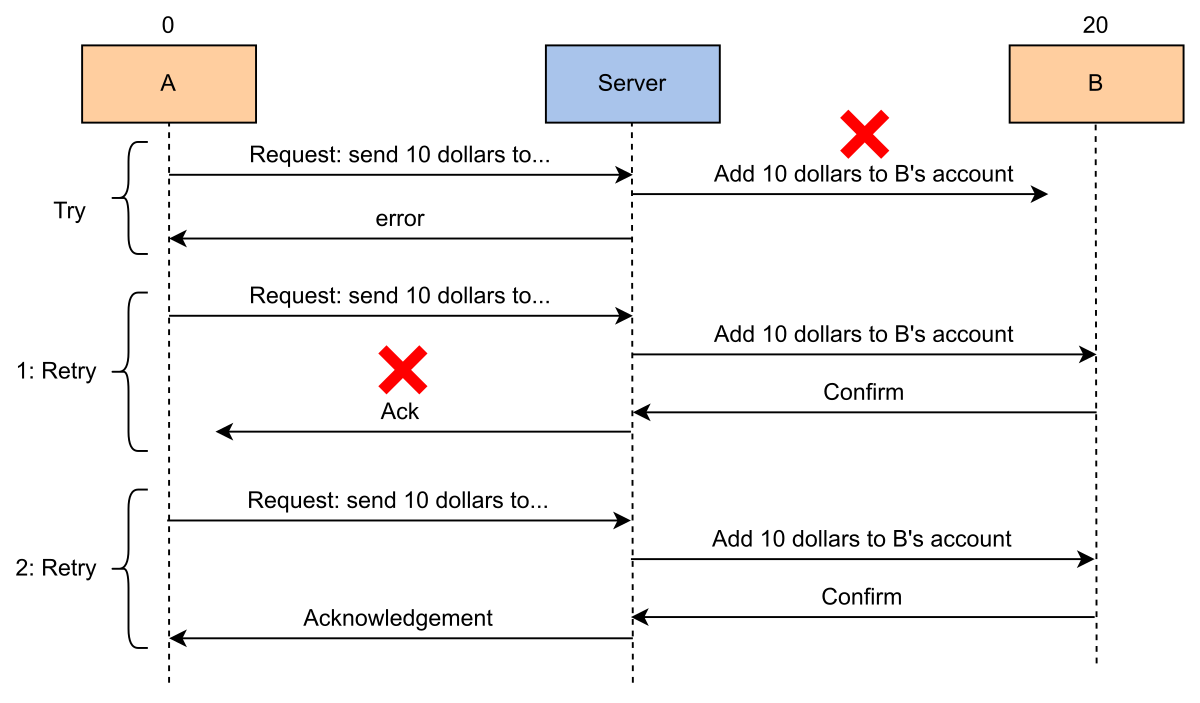
\includegraphics[width=\textwidth]{Images/chapter_23/section_4856850956156928/5715482703560704.png}
 \caption{The client has received the acknowledgement, but we end up with the wrong output. 20 dollars are added to B’s account instead of 10, and 10 extra dollars are deducted from A’s account}
 \end{subfigure}
\end{figure}

We don't want the final result to change when executing the task again. This is critical in financial applications while transferring money. We require that tasks are idempotent(\hspace{0pt}\hspace{0pt} Idempotence is a characteristic of certain operations in mathematics and computer science that allows them to be applied several times without influencing the outcome.). An idempotent task produces the same result, no matter how many times we execute it. The execution of an idempotent task is shown in the following illustration:

\begin{figure}[htbp]
 \centering
 \begin{subfigure}[b]{0.48\textwidth}
 \centering
 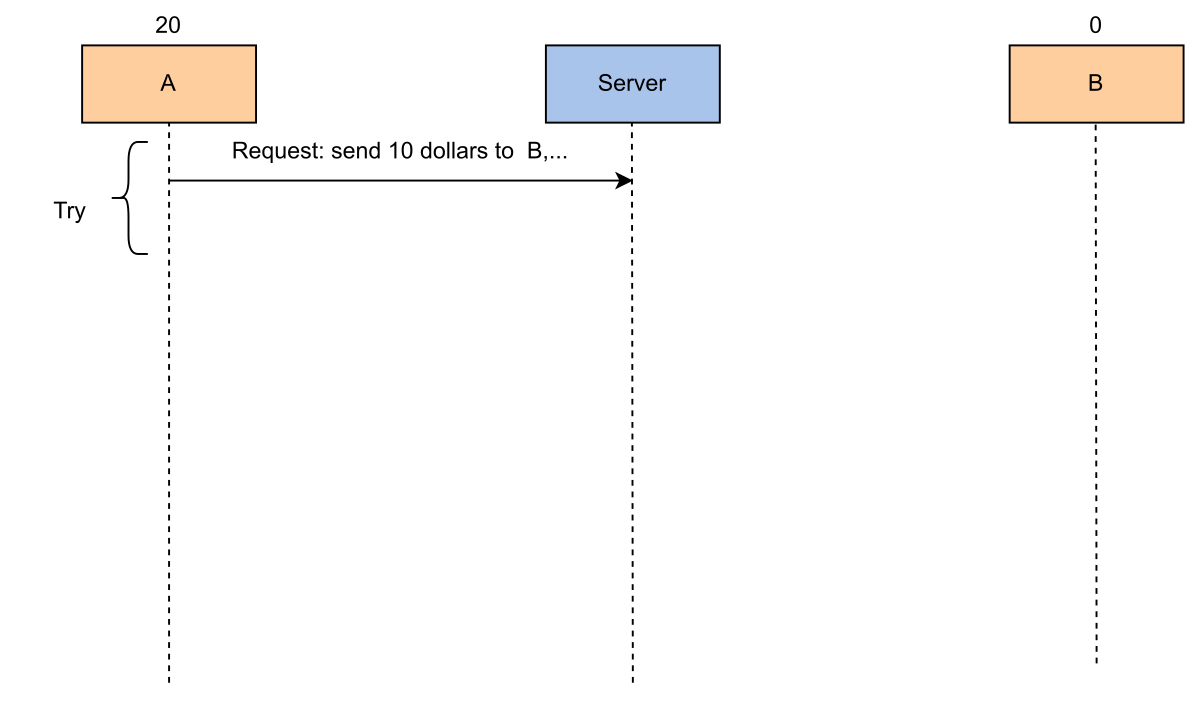
\includegraphics[width=\textwidth]{Images/chapter_23/section_4856850956156928/6328248908906496.png}
 \caption{A makes a request to send 10 dollars to B with the idempotence key that is added by the application}
 \end{subfigure}
 \hfill
 \begin{subfigure}[b]{0.48\textwidth}
 \centering
 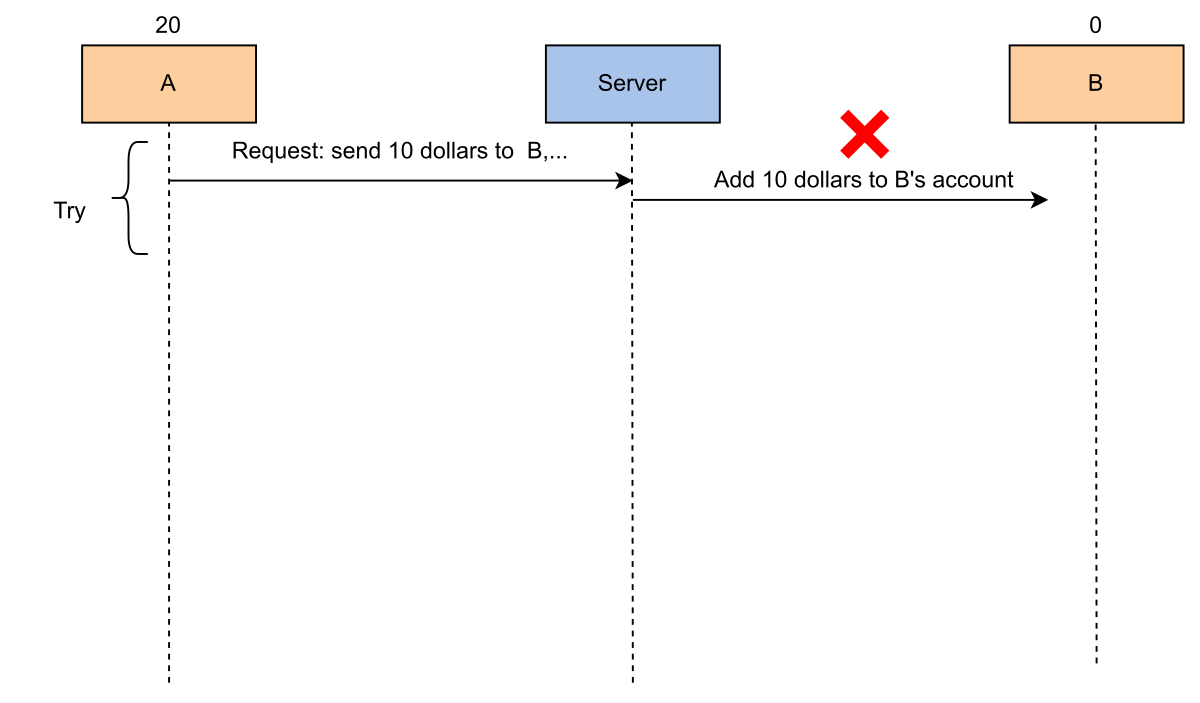
\includegraphics[width=\textwidth]{Images/chapter_23/section_4856850956156928/6704836393566208.png}
 \caption{The server starts the operation of adding 10 dollars to B’s account, which doesn’t execute successfully}
 \end{subfigure}
\end{figure}

\begin{figure}[htbp]
 \centering
 \begin{subfigure}[b]{0.48\textwidth}
 \centering
 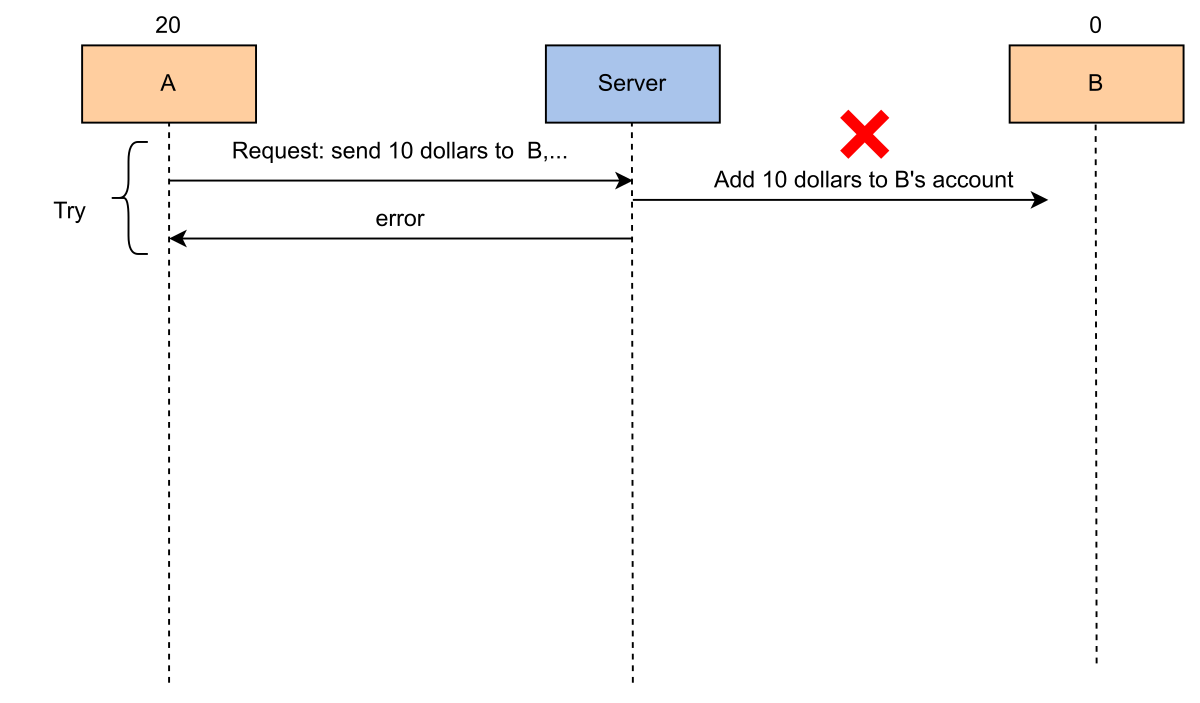
\includegraphics[width=\textwidth]{Images/chapter_23/section_4856850956156928/5900830326915072.png}
 \caption{The server sends an error message to A}
 \end{subfigure}
 \hfill
 \begin{subfigure}[b]{0.48\textwidth}
 \centering
 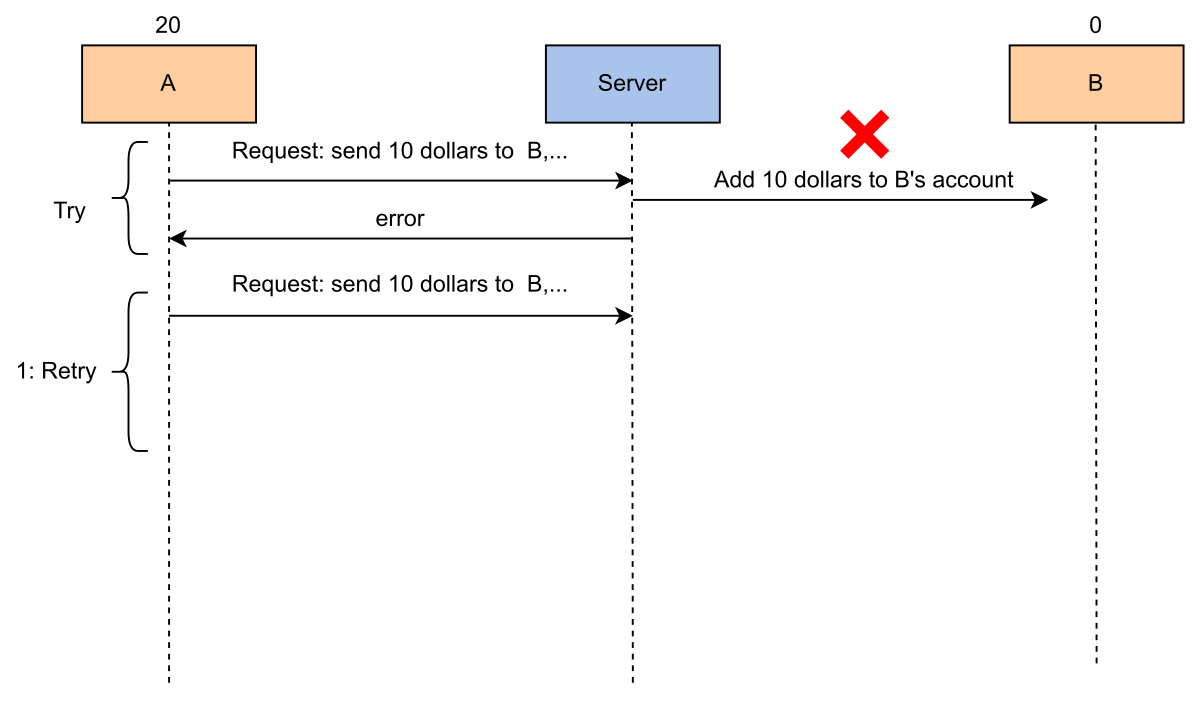
\includegraphics[width=\textwidth]{Images/chapter_23/section_4856850956156928/6211842007629824.png}
 \caption{A retries the transaction, and the same idempotence key is attached with the retried request}
 \end{subfigure}
\end{figure}

\begin{figure}[htbp]
 \centering
 \begin{subfigure}[b]{0.48\textwidth}
 \centering
 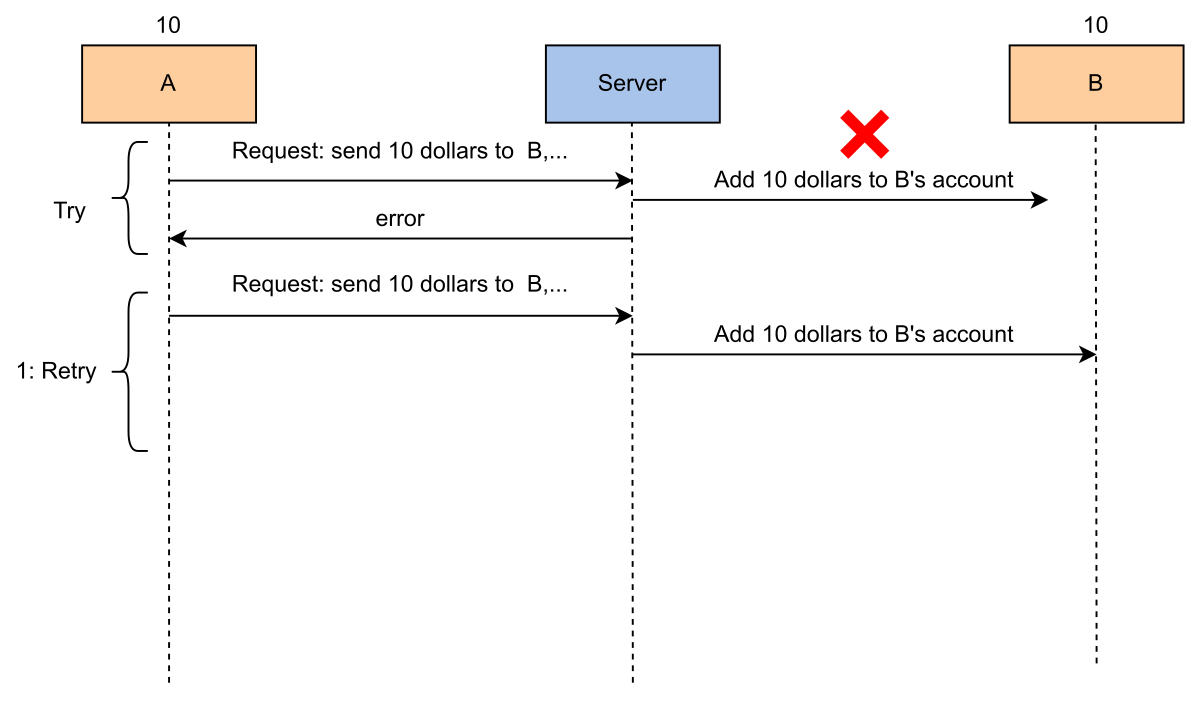
\includegraphics[width=\textwidth]{Images/chapter_23/section_4856850956156928/5784174988623872.png}
 \caption{The server starts the operation of adding 10 dollars to B’s account}
 \end{subfigure}
 \hfill
 \begin{subfigure}[b]{0.48\textwidth}
 \centering
 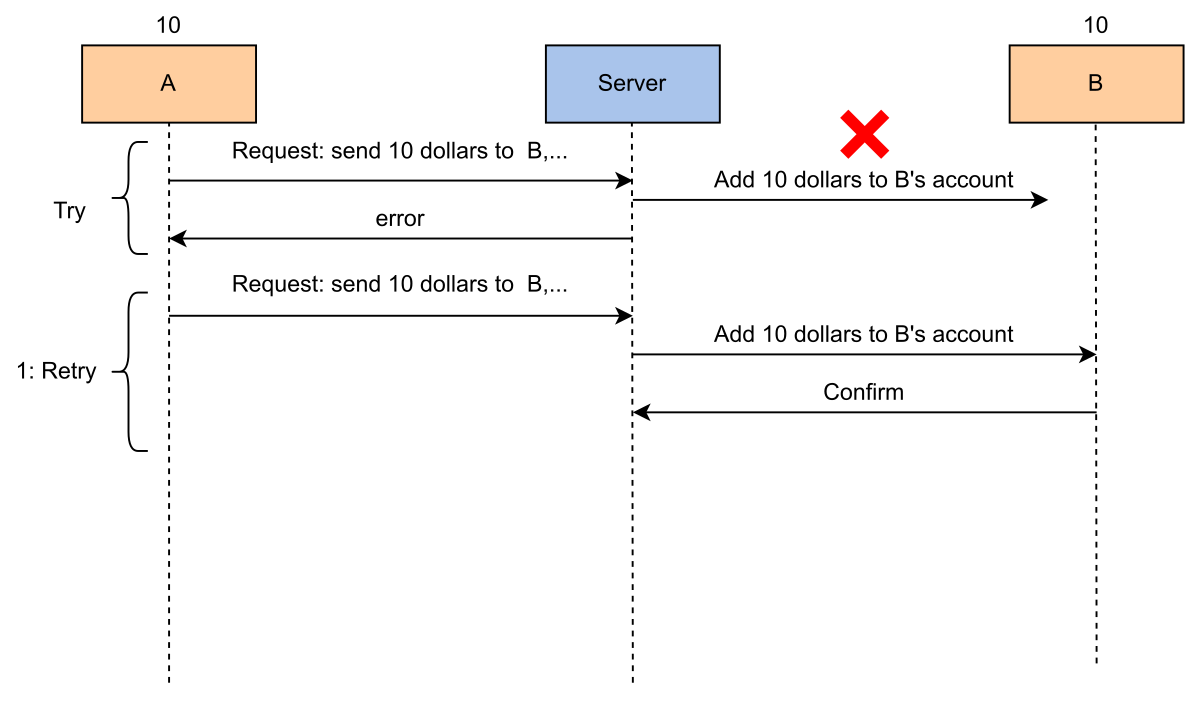
\includegraphics[width=\textwidth]{Images/chapter_23/section_4856850956156928/5229696321323008.png}
 \caption{This time the server is able to execute the operation of adding 10 dollars to B’s account successfully}
 \end{subfigure}
\end{figure}

\begin{figure}[htbp]
 \centering
 \begin{subfigure}[b]{0.48\textwidth}
 \centering
 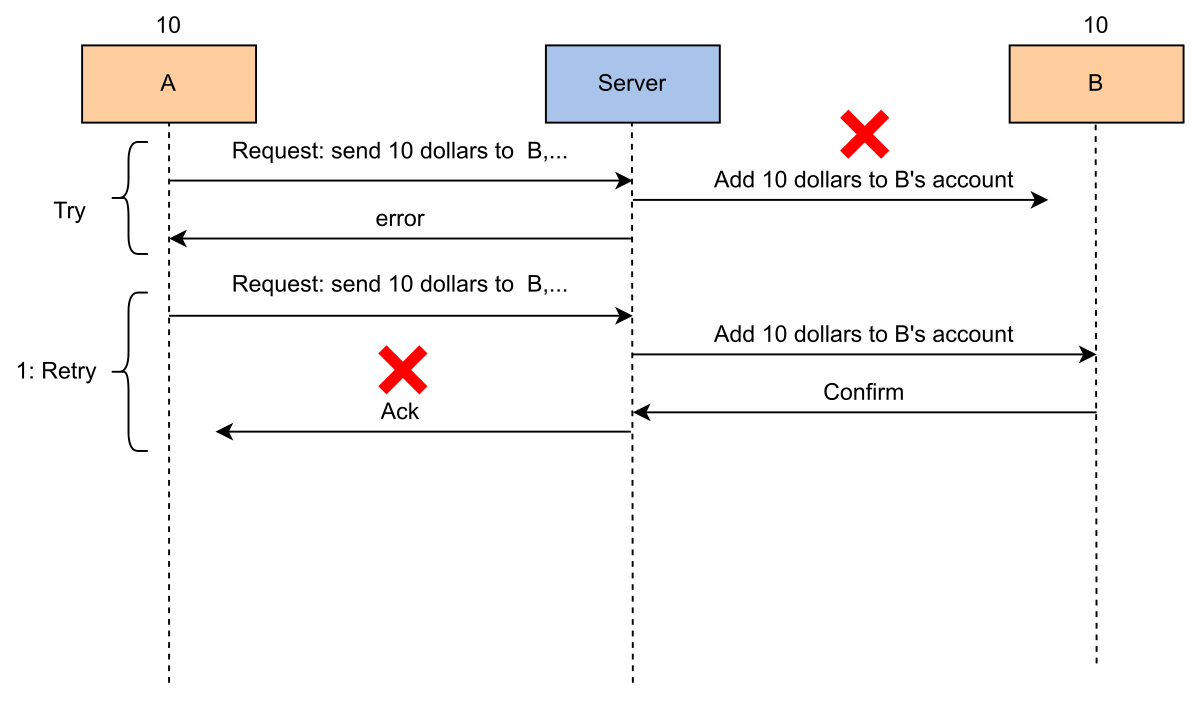
\includegraphics[width=\textwidth]{Images/chapter_23/section_4856850956156928/6293649659002880.png}
 \caption{The server sends acknowledgement to A, but it is lost due to some error}
 \end{subfigure}
 \hfill
 \begin{subfigure}[b]{0.48\textwidth}
 \centering
 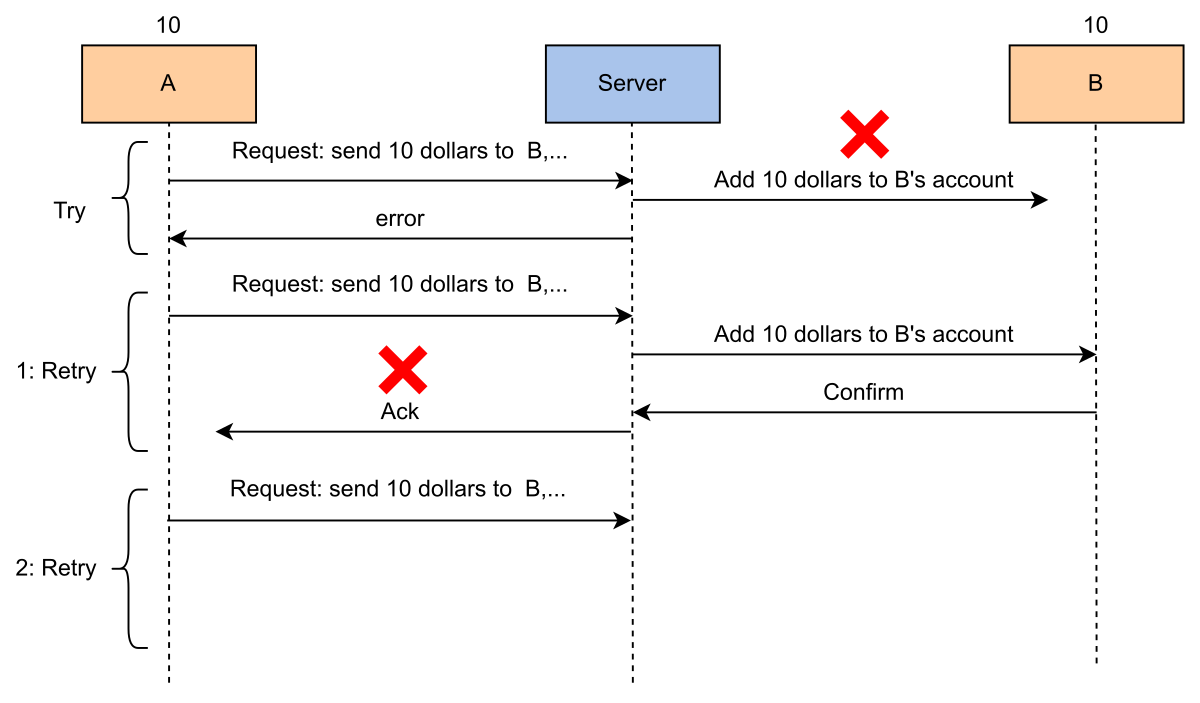
\includegraphics[width=\textwidth]{Images/chapter_23/section_4856850956156928/5534987965431808.png}
 \caption{A re-retries the transaction, and the idempotence key is also attached to the retried request}
 \end{subfigure}
\end{figure}

\begin{figure}[htbp]
 \centering
 \begin{subfigure}[b]{0.48\textwidth}
 \centering
 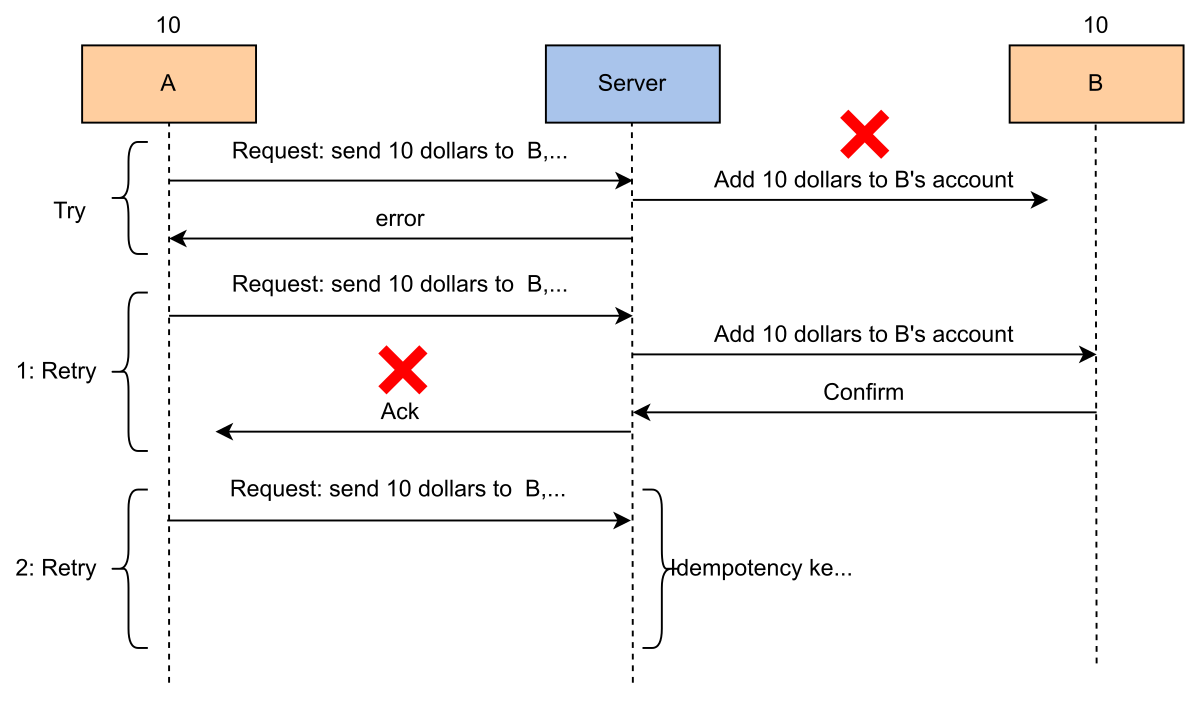
\includegraphics[width=\textwidth]{Images/chapter_23/section_4856850956156928/6679681923547136.png}
 \caption{The server found the idempotency key, so it doesn't add 10 dollars to B's account again}
 \end{subfigure}
 \hfill
 \begin{subfigure}[b]{0.48\textwidth}
 \centering
 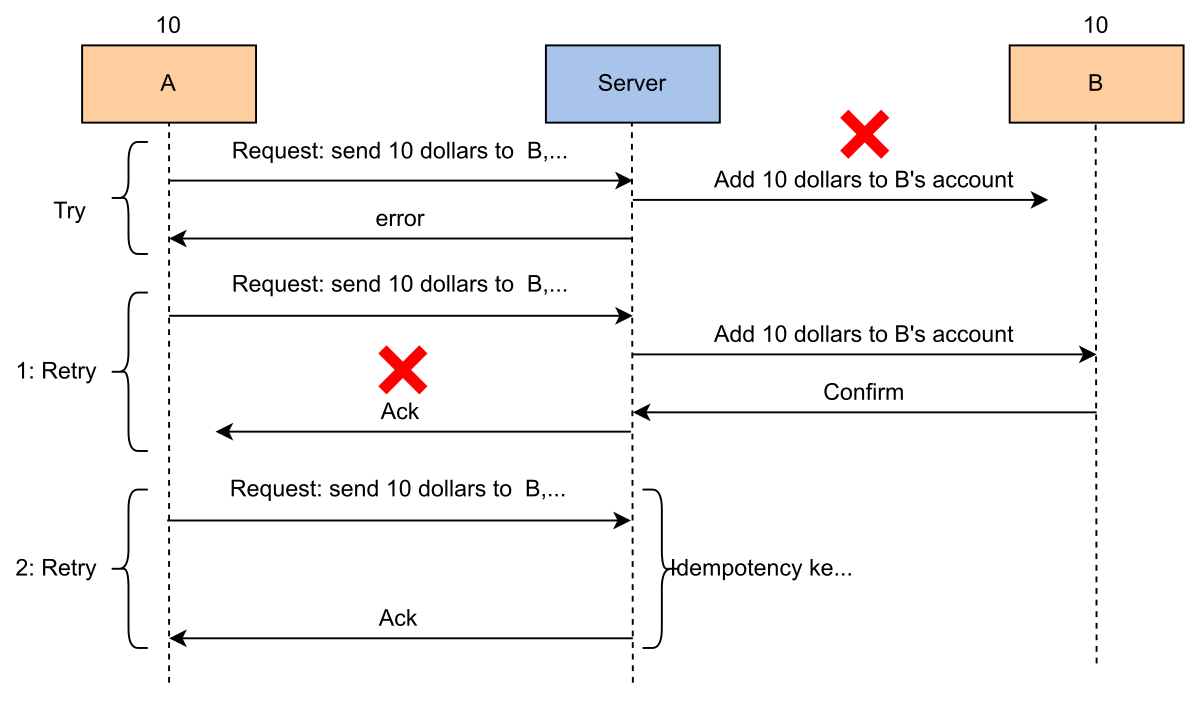
\includegraphics[width=\textwidth]{Images/chapter_23/section_4856850956156928/5384501719203840.png}
 \caption{The client receives an acknowledgement, and we get the correct output. A has 10 dollars and B has 10 dollars}
 \end{subfigure}
\end{figure}

Let's make the task of uploading a video to the database an idempotent operation. We don't want the video to be duplicated in the database in case the uploader didn't receive the acknowledgment. Idempotency ensures that the video is not duplicated. This property is added in the implementation by the developers where they identify the video by something (for example, its name) and overwrite the old one. This way, no matter how many times someone uploads it, the final result is the same. Idempotency enables us to simply re-execute a failed task.

\begin{quote}
\textbf{Quiz:}
\textbf{Question 1:} How should we handle task execution that can never be completed because of an infinite loop in the payload of that task?
\textbf{Answer:} We need to mark and kill such tasks. So, for this purpose, we can set

**time limits**. If it takes more than the specified execution cap value, we can kill the task. But it's challenging to differentiate between a buggy task and a long task. We can handle it at the application level where the clients take care of the long tasks by saving the state at different times. Clients can also resume from that state if the task scheduler kills that task, assuming that the task contains an infinite loop.
\end{quote}

\subsection{Schedule and execute untrusted tasks}\label{TEJbRpMikPNHzHo3K6UV7}
\\
\hfill\break
Before proceeding, let's ask ourselves a question: What are the untrusted tasks, and how should we manage them?\\
\strut \\
If you're unsure about the answer, click the ``Show Hint'' button below:\\

Untrusted tasks are the tasks where there is a chance of some malicious instructions in the task script that can affect the execution of the other tasks. The affected tasks could be those of the other tenants. Untrusted tasks can also harm the operating system or the resource on which they're executed.

Programs have latent bugs and might have malicious intent. When using task schedulers, we should be careful that one task does not impact other tasks negatively. If we provide infrastructure as a service, security is an essential component. This is because it becomes easier for tenants to harm each other's tasks by executing malicious code in the shared environment. Execution of malicious code can also damage our infrastructure. So, we need to keep the following considerations in mind:

\begin{itemize}
\item
\protect\phantomsection\label{8QNzrovJ-VjArhcF4pvPB}
Use appropriate authentication and resource authorization.
\item
\protect\phantomsection\label{7s15UcUWmo1iai0NAZZpl}
Consider code sandboxing using dockers or virtual machines.
\item
\protect\phantomsection\label{Bk8oCDEBauFkgueH0NT5V}
Use performance isolation between tasks by monitoring tasks' resource utilization and capping (or terminating) badly behaving tasks.
\end{itemize}

\begin{quote}
\textbf{Quiz:}
\textbf{Question 1:} What happens when the same task fails multiple times?
\textbf{Answer:} We can use a dead-letter queue facility to isolate repeatedly failing tasks.
\end{quote}

Now, let's evaluate the design of our distributed task scheduler in the next lesson.

% End of section content